\chapter{Einleitung}
\label{chap:einleitung}
Heutzutage ist die Menschheit darauf fokussiert, die komplette Welt zu digitalisieren. Dabei
existiert ein Grundsatz, alles, was digitalisiert werden kann, soll digitalisiert werden. Um dies
zu realisieren, ist es von Nöten, überall Hardware und Software zu verbinden. Sei es nun das
Handy, mit welchem durch nur einem klick die Bankdaten angezeigt werden können, oder ein
selbstfahrendes Auto, welches einen Anwender selbstständig zum Ziel fährt. Dies sind nur zwei
bespiele von einer unendlich langen Liste. Hinter diesen technischen Wundern stecken meist
mehrere Tausend kleiner Mikrocomputern und Mikrocontrollern, die dann mittels Software zusammen
interagieren. Die Kombination dieser zwei Komponenten werden durch den Oberbegriff „Embedded
System“ oder auch zu Deutsch ein „Eingebettetes System“ definiert.
\newline
\newline
Embedded Systems können dabei grundsätzlich zwischen zwei Plattformen unterschieden werden:
\begin{itemize}
    \item Deeply Embedded System
    \item Open Embedded System
\end{itemize}
\newline
\newline
Deeply Embedded Systems sind die wesentlichen Bausteine des Internet of Things
\cite{HochschuleniederrheimDeeply}. Die Anwendung,
die bei Deeply Embedded Systems implementiert wird, basiert auf speziell angepassten
Echtzeitbetriebssystemen, den Programmiersprachen C oder C++ und ganz speziellen GUI-Frameworks
wie zum Beispiel TouchGFX.
\newline
\newline
Anders als bei den Deeply Embedded Systems, die sehr auf speziellen Technologien aufbauen, bieten
Open Embedded Systems eine höhere Flexibilität in Sachen Technologien an. Dem Programmierer ist
also die Möglichkeit gegeben, unterschiedliche Technologien sowohl als auch unterschiedliche
Programmiersprachen zu verwenden. Dort gilt bis dato die Kombination von C++ und Qt für
GUI-lastige Systeme als „State of the Art“.
\newline
\newline
Die Konstellation zwischen C++ und Qt hat bislang auch funktioniert, jedoch kommt dieser Ansatz
auch mit Problemen mit sich, denn die höheren Entwicklungszeiten für die Entwicklung von C++
Anwendungen sowie die geringe Verfügbarkeit von Experten auf dem Arbeitsmarkt sorgen für
schlechtere Qualität und längere Produktionszeiten.
\newline
\newline
Um diesen Problemen zu entgegnen, soll in dieser Abschlussarbeit ein anderer Ansatz betrachtet
werden. Und zwar könnten sowohl die Anwendungsschicht als auch die Persistenzschicht als .Net
Core Anwendungen implementiert werden. Als GUI-Technologie soll dabei die neue
Microsofttechnologie namens \emph{Blazor} als Qt Ersatz zum Einsatz kommen. Somit kann erreicht
werden, die komplette Codebasis mit .Net Core auszutauschen und eine Programmier-freundlichere
Umgebung für Entwickler im Open Embedded Systems zu erschaffen.
\section{Aufgabenstellung}
\label{sec:aufgabenstellung}
Das Ziel dieser Arbeit ist die Entwicklung eines Blazor-basierten Frontend auf einem Raspberry Pi
4 um einen aussagekräftigen Vergleich zwischen den Technologien schaffen zu können und um eine
mögliche verdrängung mittels Blazor zu demonstrieren. Dazu soll
zunächst begutachtet werden, wie der momentane Stand der Technik für Open Embedded Systems ist,
um anschließend das gleiche Verhalten mittels Blazor zu reproduzieren. Insbesondere sollen dabei
verschiedene Aspekte, wie zum Beispiel das Verhalten zur Laufzeit, dieses Ansatzes überprüft werden.
\begin{figure}[h]
    \centering
    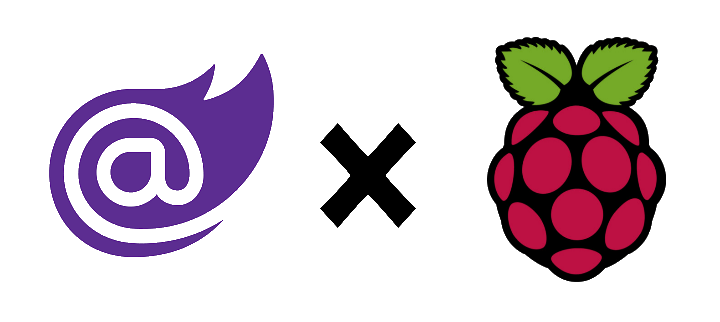
\includegraphics[width=0.8\textwidth, center]{Einleitung/blazorxraspberry}
    \caption[Blazor mit Raspberry Pi]{Blazor mit Raspberry Pi}
    \label{img:blazorxraspberry}
\end{figure}
